\documentclass{article}
\usepackage{enumerate}
\usepackage{graphicx}
\usepackage{subcaption}
\usepackage{hyperref}
\usepackage{epstopdf}
\usepackage{amsmath}
\usepackage{geometry}
\usepackage{color}
\usepackage{makecell}
\usepackage{xcolor}
\usepackage{booktabs}
\geometry{left=2.5cm,right=2.5cm,top=1.5cm,bottom=2cm}

\bibliographystyle{ieeetr}

\title{Building a database of Alzheimer's patients}
\author{Jicheng Lu}
\date{}

\begin{document}
\maketitle
%\tableofcontents

\section{Introduction}
\paragraph{}
At this stage, we need to build a database of the patients who have diagnosed with Alzheimer's disease. However, due to the privacy issue and limited access to the existing database, we cannot obtain enough data, especially the individual patient's data. We need to find an alternative method that is able to generate an arbitrary number of patient data.

\section{Method}
\paragraph{}
The solution introduced here is to generate "fake" data based on the aggregated patient data. In other words, we can sample multiple data points from the group distributions. \\

For example, suppose we want to have patients with different ages. We first collect the statistical data from relevant medical studies, such as the distribution of age ranges (60\% for 80-89, 30\% for 70-79, 10\% for 60-69). Then we can sample our patient data based on this distribution. One possible result can be 60 patients with age 80-89, 30 patients with age 70-79, 10 patients with age 60-69. We can apply this strategy to other attributes, such as gender, years of education, willingness, MMSE score, etc.


\section{Evaluation}
\paragraph{}
Basically, there are two ways of evaluating the rationality of the generated data:

\begin{itemize}
  \item Subjective evaluation: The data is evaluated by doctors or physicians based on their experience.
  \item Model evaluation: A classification model is trained based on the generated data and used to evaluate future data. 
\end{itemize}

For the second approach, we can first collect statistical data from Alzheimer's study and non-Alzheimer's study (e.g., other dementia diseases), respectively. Then we can train the model with more reliability.


\section{Issues}
\paragraph{}
Here we list several possible issues when sampling data:

\begin{itemize}
  \item What attributes do we need for each patient? e.g., age, race, gender, MMSE, etc.
  \item Is there any relationship between attributes?  e.g. age vs stroke history, etc.
  \item How do we connect the generated data with the criteria?
\end{itemize}


\section{Resources}
\paragraph{}
There are two resources I have found. Both of them contain a collection of statistical data from AD-related studies.

\begin{itemize}
  \item GAAIN: http://www.gaain.org/
  \item NACC: https://www.alz.washington.edu/WEB/demoDx.html
\end{itemize}

\section{Examples of Data Source}
\paragraph{}
Here we give some examples from the websites mentioned above. 

\subsection{GAAIN}
\paragraph{}
For GAAIN (i.e, Global Alzheimer’s Association Interactive Network), the data is built-in, so we can only check them in their interface. The interface is called "The Interrogator" (register an account to log in). Fig. \ref{f:gaain} gives the general picture after we log in. It contains a number of AD-related studies from all over the world. 

\begin{figure}[!hbt]
\centering
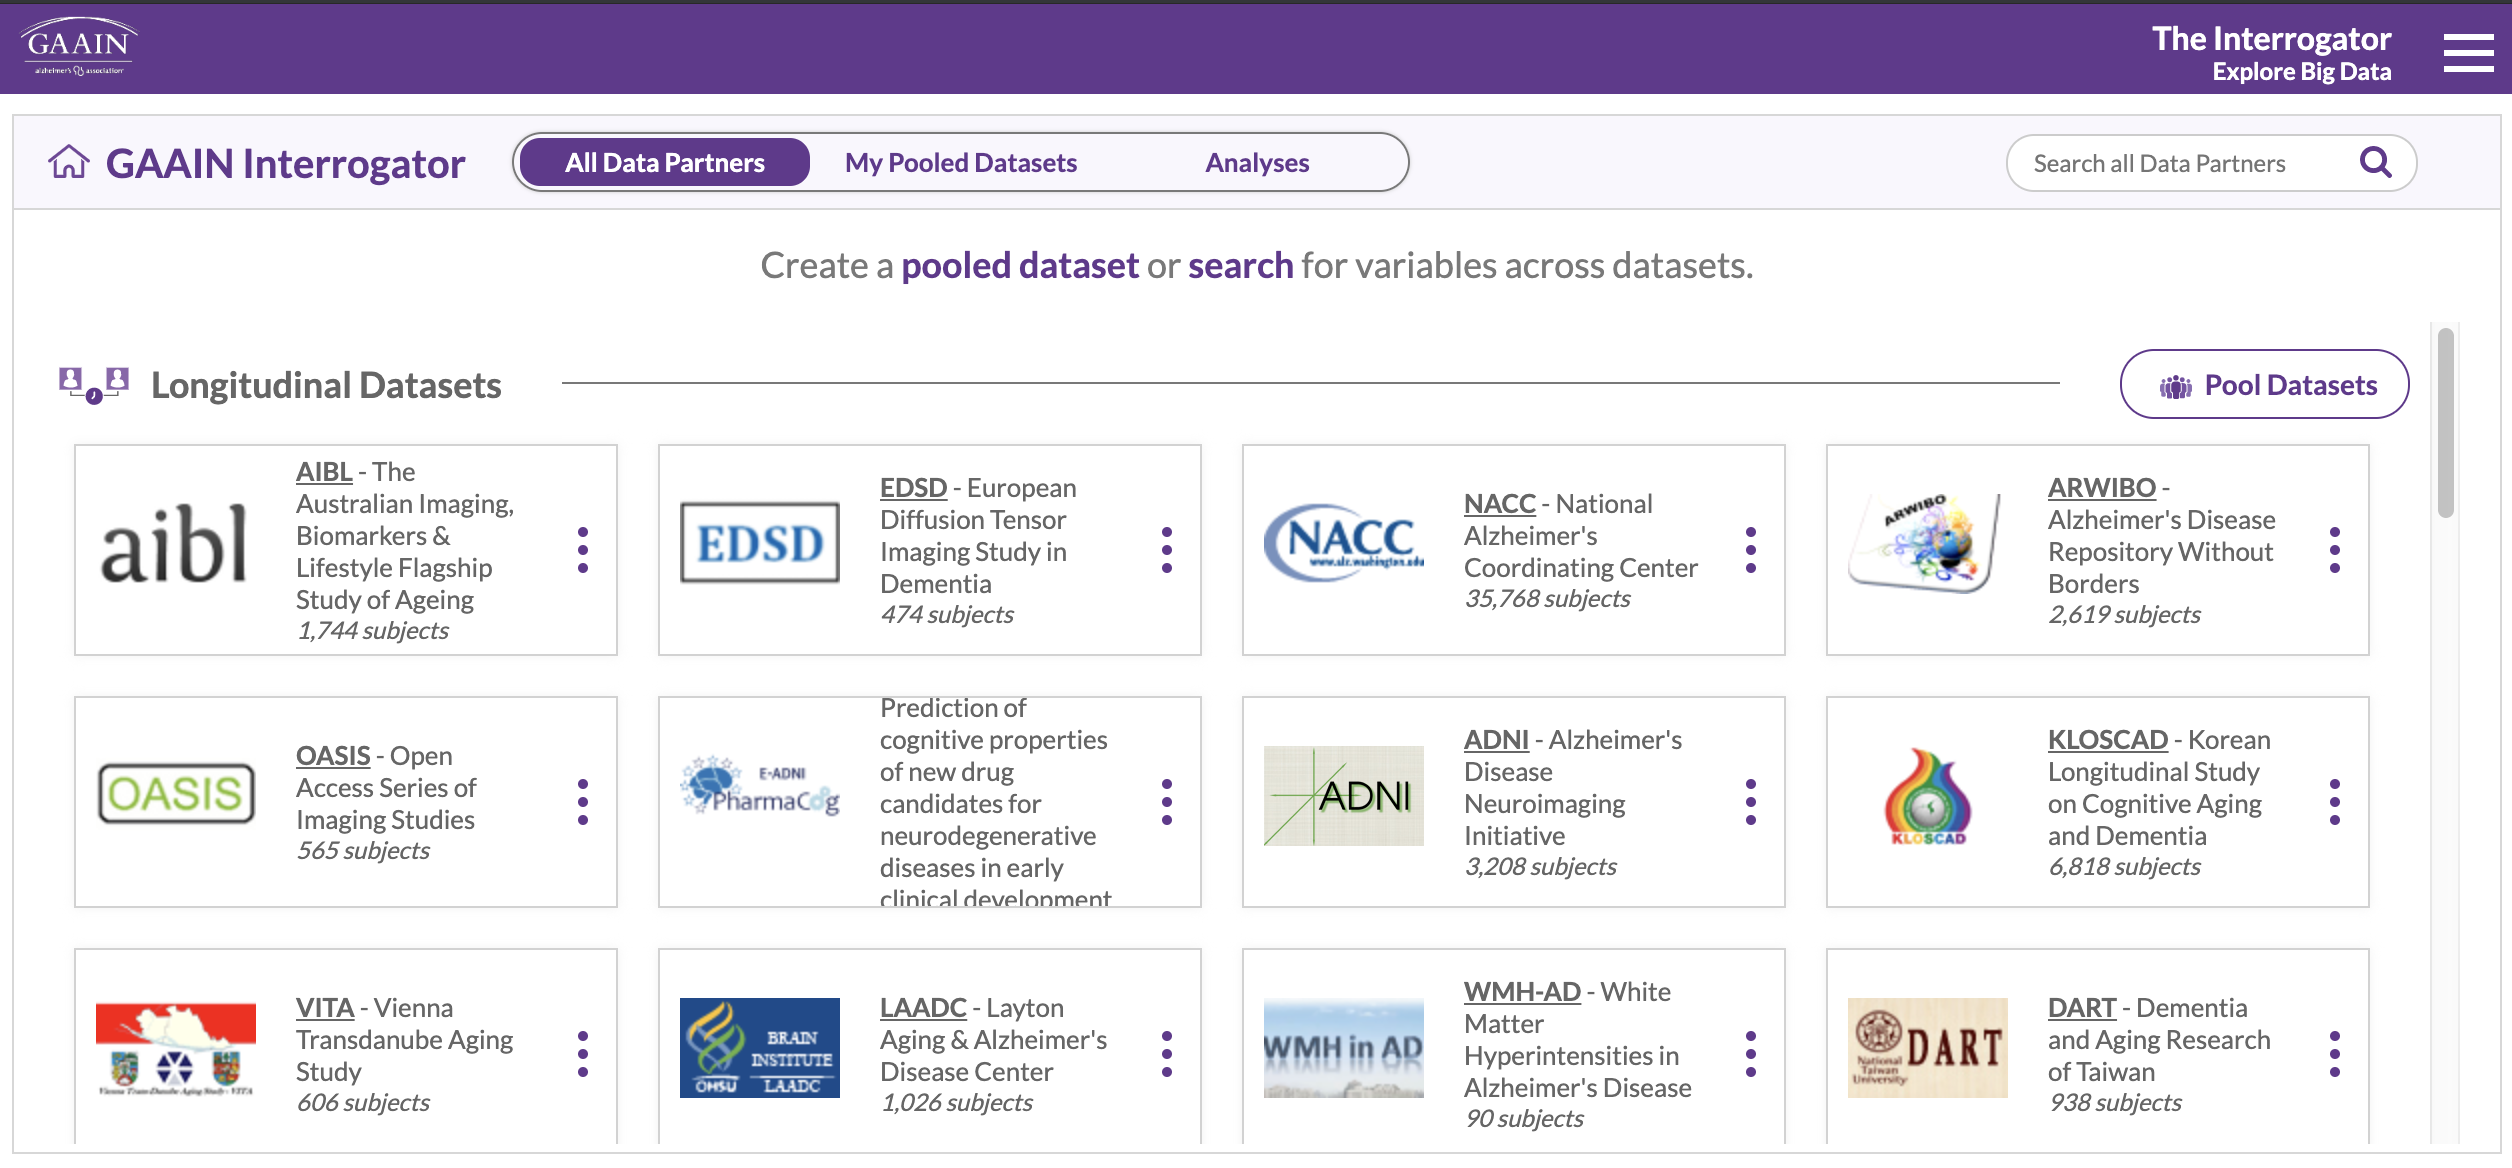
\includegraphics[width=11cm, height=6cm]{figs/gaain.png}
\caption{The Interrogator of GAAIN.}
\label{f:gaain}
\end{figure}

After we select a study, we can observe the statistical data it contains. Fig. \ref{f:aibl} presents the dataset of AIBL, a medical study from Australia. At the left hand side, we can select different variables and the results are shown at the right side. For example, Fig. \ref{f:aibl} shows the gender distribution of the subjects. We can also get the medical data, such as MMSE, medical history, etc.

\begin{figure}[!hbt]
\centering
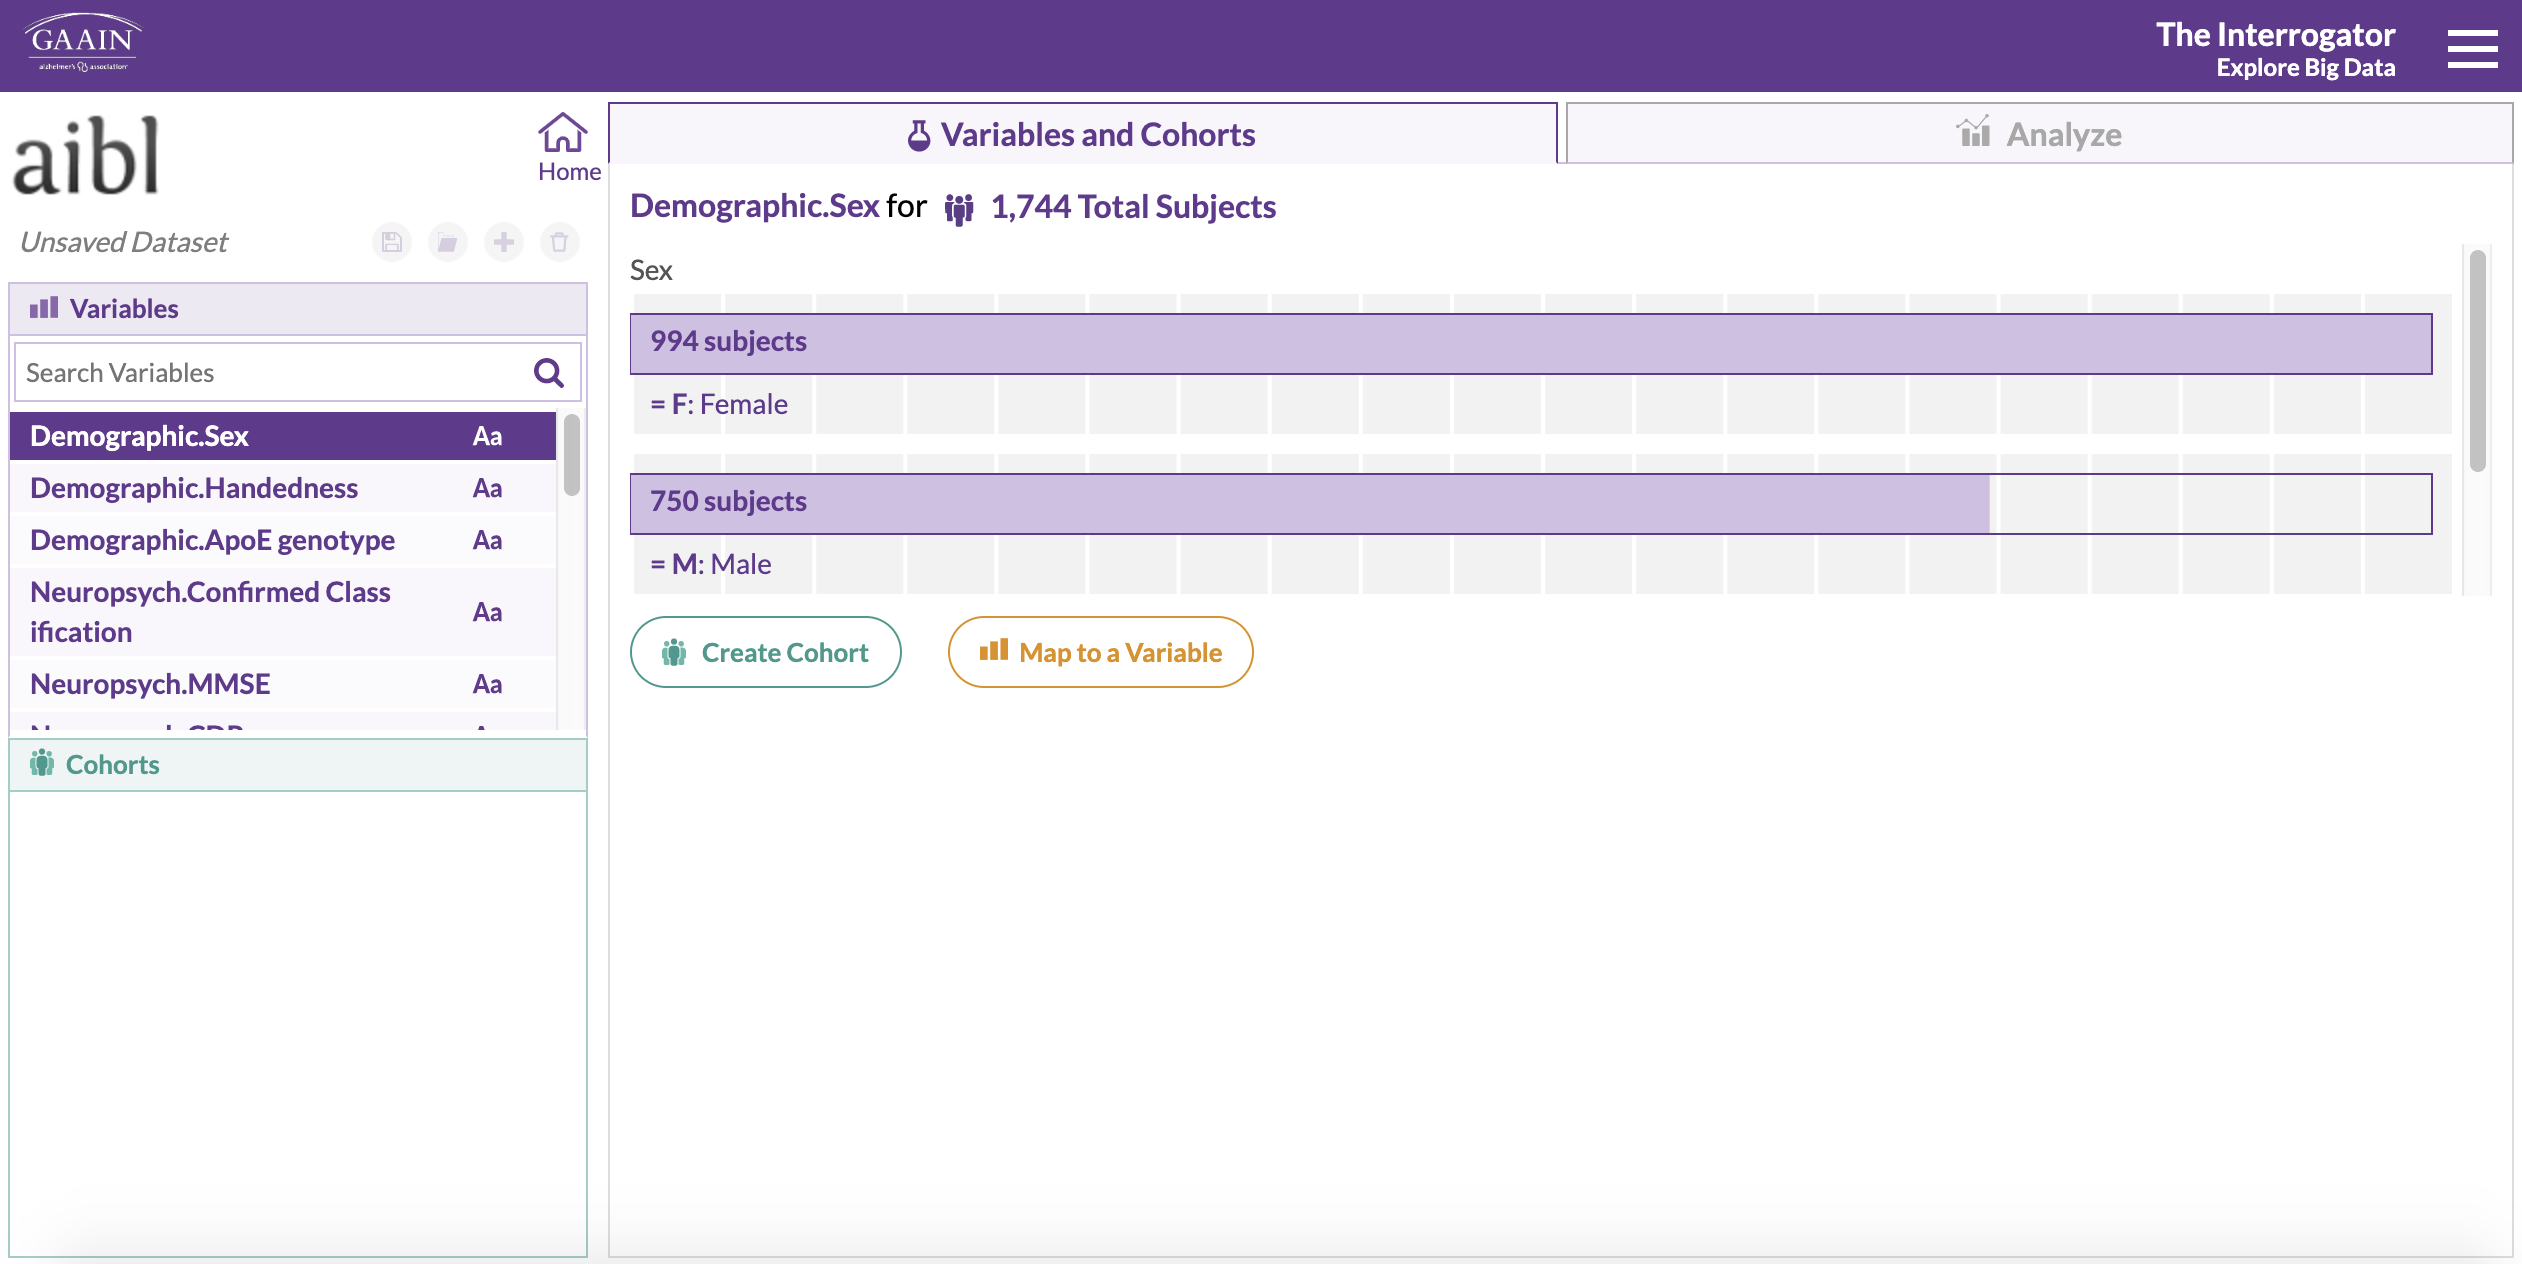
\includegraphics[width=12cm, height=6cm]{figs/aibl.png}
\caption{The dataset of AIBL.}
\label{f:aibl}
\end{figure}

\newpage
\subsection{NACC}
\paragraph{}
For NACC (i.e., National Alzheimer's Coordinating Center), they have studied patients with not only the Alzheimer's disease but also the other cognitive illness, such as Parkinson's disease, vascular brain injury, etc. Currently, we can get direct access to the UDS summary data, which contains the subject demographics as well as cognitive status (Fig. \ref{f:nacc}). The UDS dataset was contributed by the Alzheimer’s Disease Centers from 2005 to present. There are also other relevant data on NACC. For more details, please use the link provided above.

\begin{figure}[!hbt]
\centering
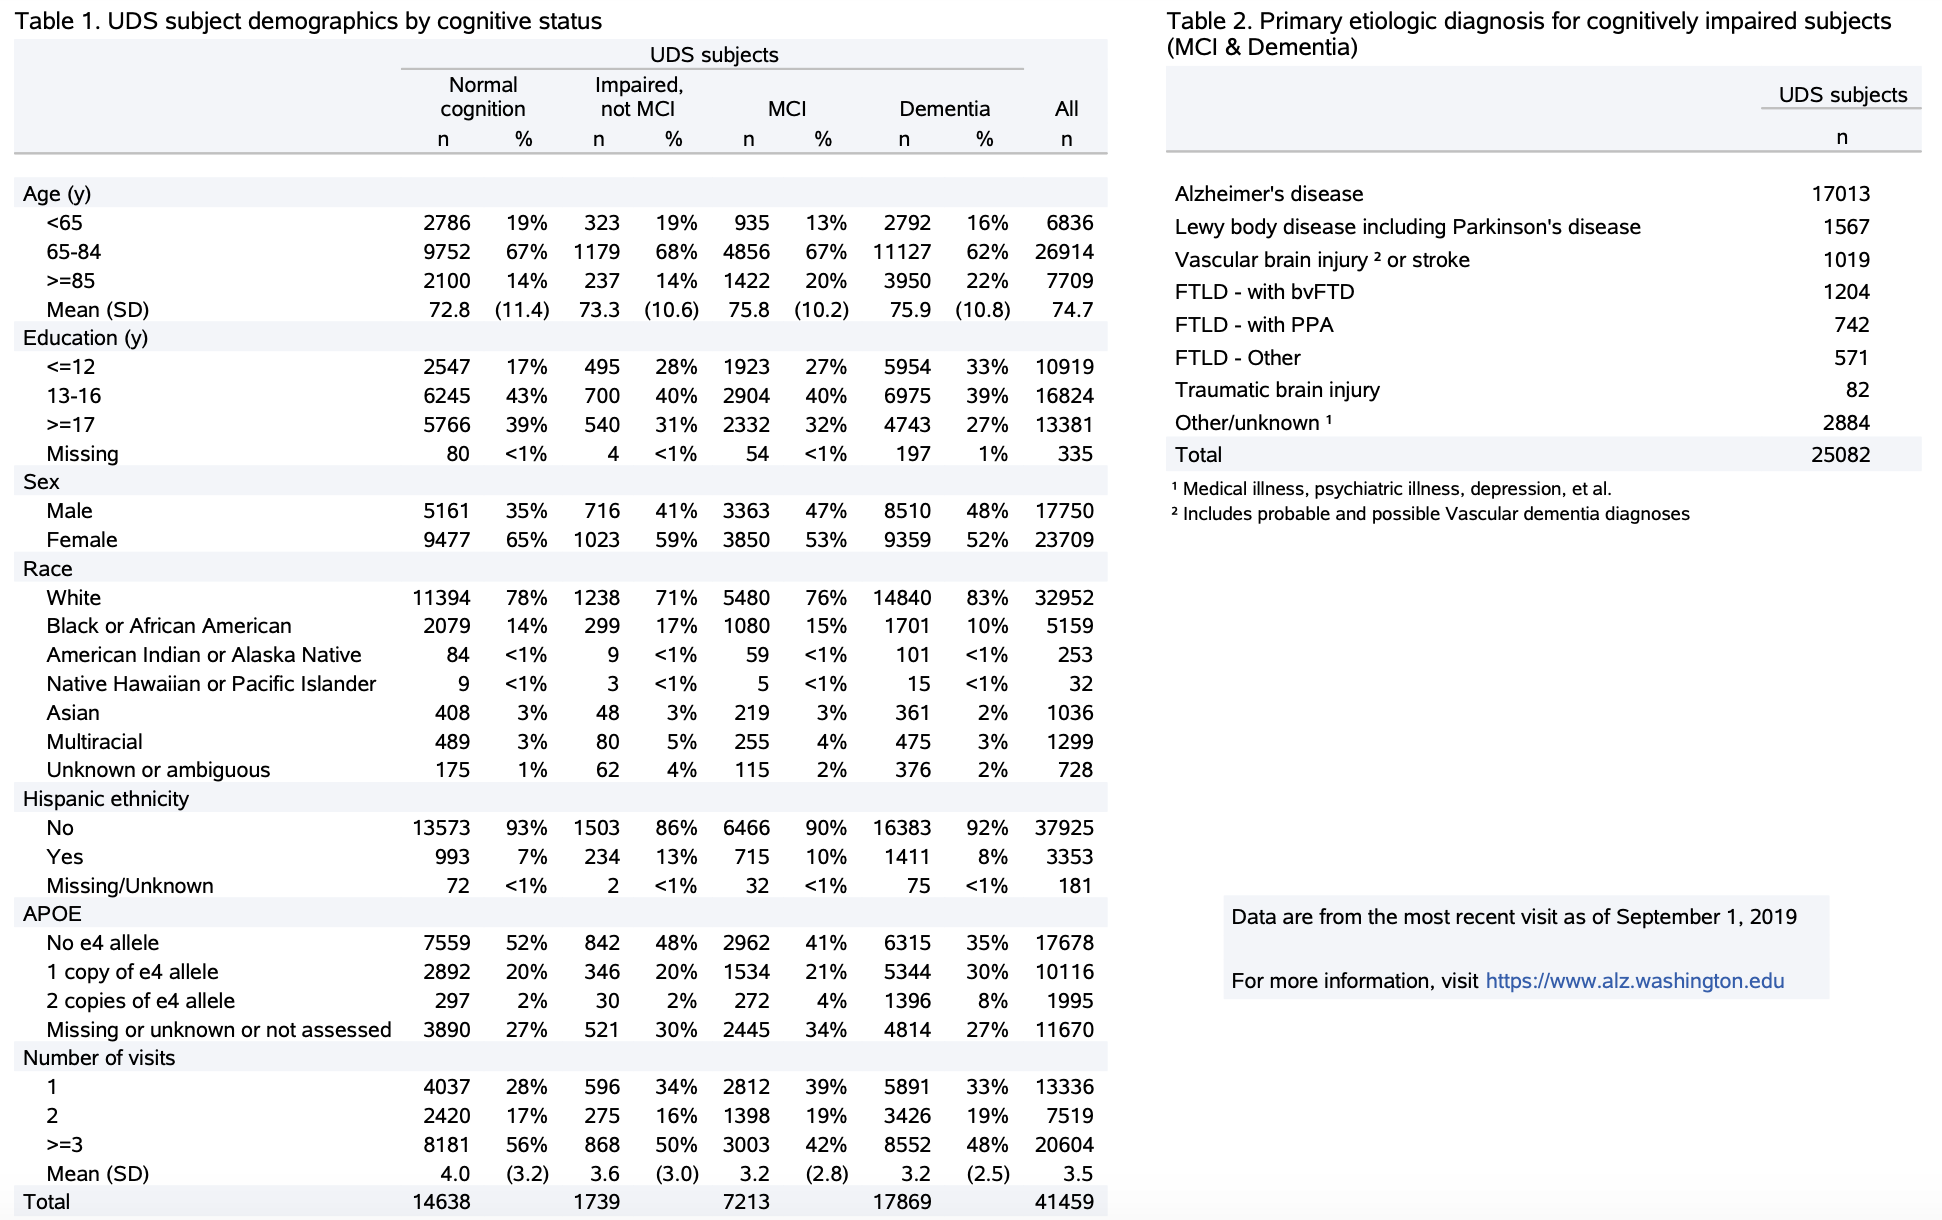
\includegraphics[width=11cm, height=6cm]{figs/nacc.png}
\caption{The UDS dataset of NACC.}
\label{f:nacc}
\end{figure}

Moreover, we can request the custom data from NACC. The keywords that can be selected belong to the following categories:

\begin{itemize}
  \item Clinical Diagnosis, e.g., Alzheimer's disease, Lewy body dementia, etc.
  \item Clinical Measures and Symptoms, e.g., blood pressure, Hachinski ischemic score, etc.
  \item Neuropsychological Testing, e.g., MMSE, composite scores, etc.
  \item Demographics, e.g., sex, race, age, etc.
  \item Subject health history, e.g., smoking, alcohol, etc.
  \item Neuropathology / Death, e.g., Lewy bodies, Neuritic plaques, etc.
  \item Genetics and Biomarkers, e.g., MRI, PET, etc.
  \item Study Design, e.g., cross-sectional, longitudinal, etc.
\end{itemize}

The entire keywords are attached with this proposal. \\

\section{Examples of Generated Data}
\paragraph{}
In this section, we present several examples of generated data using the UDS data from NACC (Fig. \ref{f:nacc}). First, we introduce the method in which we generate the patient data. As we observe from the data, we know that there is no interaction between different attributes (i.e., age, sex, race, ethnicity, years of education, etc.). For an instance, we cannot get one person's age based on his/her race and vice versa. Thus, we treat each attribute independently. \\

The main idea is to use the Bayes formula (Eq. \ref{e:bayes}). We want to get the diagnosis from the given attributes. The diagnosis classes are: "normal", "impaired, not MCI", "MCI", "dementia".

\begin{equation}
\label{e:bayes}
	P(diagnosis | attributes) = \frac{P(diagnosis) \times P(attributes | diagnosis)}{P(attributes)}
\end{equation}

Since all the attributes are independent, we compute the attribute-related components as follows. We denote the attributes as $a_1, a_2, ..., a_n$.

\begin{align}
	P(attributes) & = P(a_1) P(a_2) ... P(a_n) \\
	P(attributes | diagnosis) & = P(a_1 | diagnosis) P(a_2 | diagnosis) ... P(a_n | diagnosis)
\end{align}

Here we randomly generate 10,000 "fake" patients data, and assign diagnosis to each using Eq. \ref{e:bayes}. Fig. \ref{f:gen} gives the basic layout of part of the data.

\begin{figure}[!hbt]
\centering
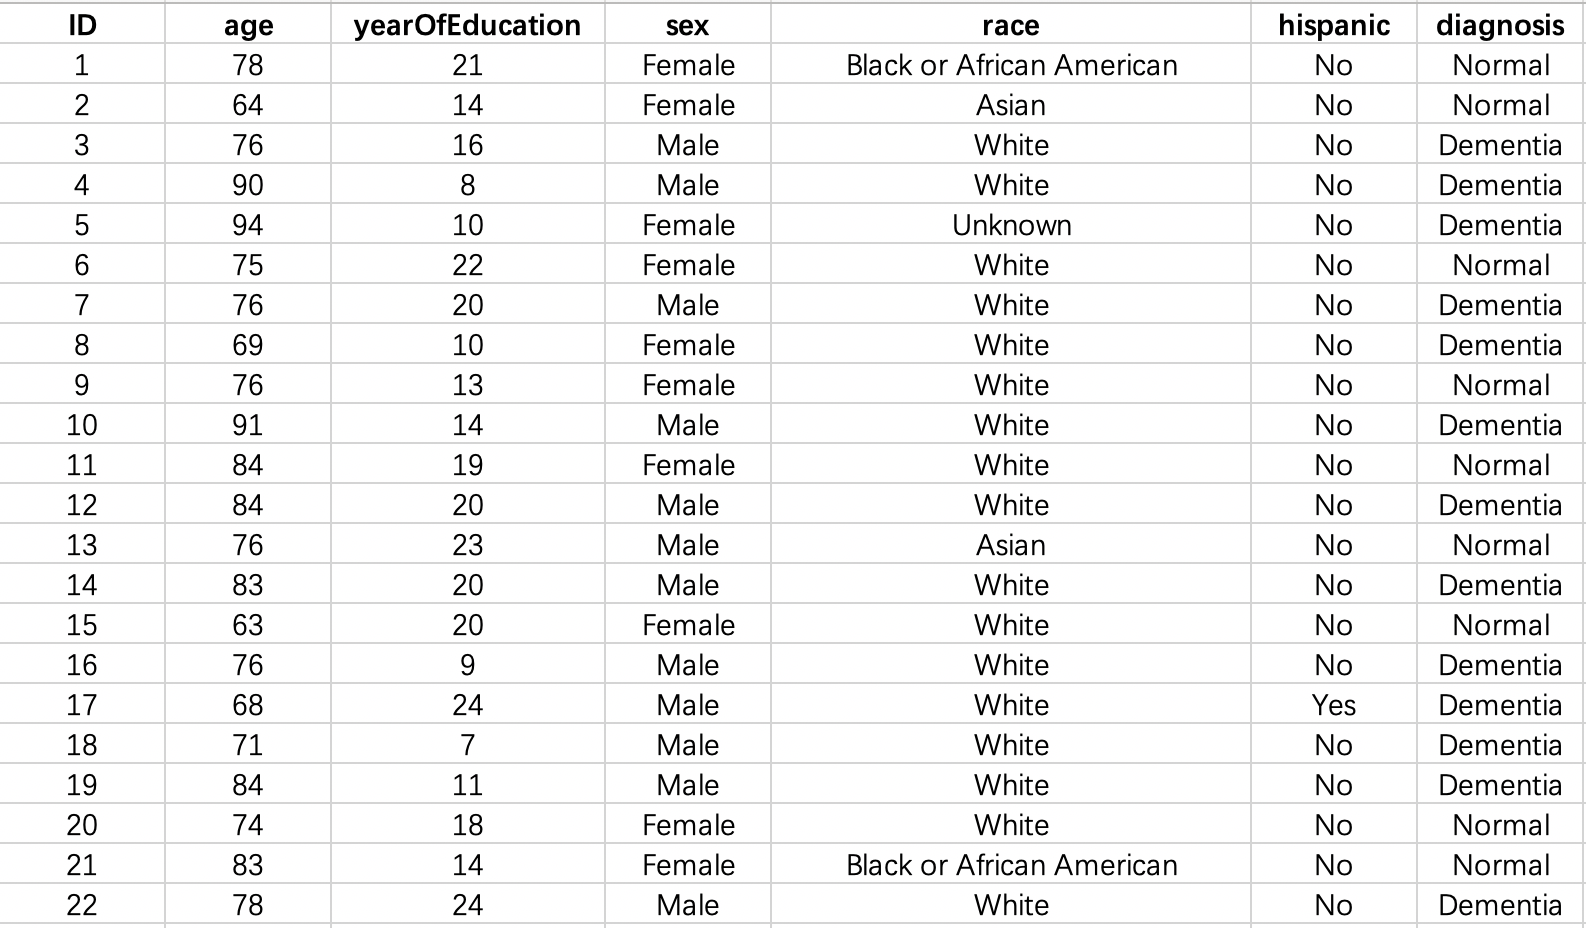
\includegraphics[width=11cm, height=6cm]{figs/genData.png}
\caption{The layout of the generated data.}
\label{f:gen}
\end{figure}

To validate the correctness of the generated data, we compare the distributions of several attributes between the generated data and raw data.

\begin{table}[!hbt]
  \centering
  \caption{Distribution comparison of "age".}
  \begin{tabular}{c|c|c}
  \toprule
  Age & raw distribution($\%$) & generated distribution($\%$) \\
  \midrule
  $<$ 65 & 16.5 & 16.2 \\
  65-84 & 64.9 & 65.2 \\
  $\geq$ 85 & 18.6 & 18.6 \\
  \bottomrule
  \end{tabular}
\end{table}

\begin{table}[!hbt]
  \centering
  \caption{Distribution comparison of "years of education".}
  \begin{tabular}{c|c|c}
  \toprule
  Education (y) & raw distribution($\%$) & generated distribution($\%$) \\
  \midrule
  $\leq$ 12 & 26.3 & 26.7 \\
  13-16 & 40.6 & 40.9 \\
  $\geq$ 17 & 32.3 & 32.3 \\
  \bottomrule
  \end{tabular}
\end{table}

\begin{table}[!hbt]
  \centering
  \caption{Distribution comparison of "sex".}
  \begin{tabular}{c|c|c}
  \toprule
  Sex & raw distribution($\%$) & generated distribution($\%$) \\
  \midrule
  Male & 42.8 & 42.5 \\
  Female & 57.2 & 57.5 \\
  \bottomrule
  \end{tabular}
\end{table}

\newpage
Moreover, we check the distribution of the generated diagnosis. We notice that there is zero diagnosis of "Impaired, not MCI" and "MCI". This may be because the original probabilities of these two diagnoses are much smaller, compared to the other two cases.

\begin{table}[!hbt]
  \centering
  \caption{Distribution comparison of "diagnosis".}
  \begin{tabular}{c|c|c}
  \toprule
  Diagnosis & raw distribution($\%$) & generated distribution($\%$) \\
  \midrule
  Normal & 35.3 & 38.2 \\
  Impaired, not MCI & 4.2 & 0.0 \\
  MCI & 17.4 & 0.0 \\
  Dementia & 43.1 & 61.8 \\
  \bottomrule
  \end{tabular}
\end{table}

\section{Summary}
\paragraph{}
This proposal introduces the idea about generating "fake" patients data from the aggregated data. The data is generated using Bayes formula, where each attribute is treated independently. We provide several examples of the generated data, and we observe that they follow the similar distributions with the raw data.

\end{document}












